\section{Errors}

The error boundaries for the classifiers were obtained
for both the Chernoff and Bhattacharyya Bounds \cite{duda2012pattern}.

For the Chernoff Bounds, the following equations were employed.

\begin{align*}
 \min[a,b] & \leq a^\beta b^{1-\beta}  \quad \text{for } a,b \geq 0 \text{ and } 0\leq \beta \leq 1  \\
 P(\text{error}) & \leq P^\beta (\omega_1) P^{1-\beta} (\omega_2) \int p^\beta (x | \omega_1)p^{1-\beta}(x|\omega_2)dx  \text{ for } 0 \leq \beta \leq 1\\
\int p^\beta &(x | \omega_1)p^{1-\beta}(x|\omega_2)dx  = \exp(-k(\beta)) \\
k(\beta) &= \frac{\beta(1-\beta)}{2} (\mu_2 - \mu_1)^T \det(\beta  \Sigma_1 + (1-\beta)\Sigma_2)^{-1} (\mu_2 - \mu_1) \\
& \quad + \frac{1}{2} \ln \frac{\det(\beta \Sigma_1  + (1-\beta)\Sigma_2)}{\det(\Sigma_1)^\beta \det(\Sigma_2)^{1-\beta}}
 \end{align*}

 Likewise, for the Bhattacharyya Bounds another set of equations was utilized

\begin{align*}
 P(\text{error}) & \leq \sqrt{P{\omega_1} P(\omega_2)} \int \sqrt{p(x | \omega_1) p(x|\omega_2)} dx\\
 &= \sqrt{P{\omega_1} P(\omega_2)} \exp{-k(1/2)}\\
 k(1/2) &= \frac{1}{8}(\mu_2 - \mu_1)^T \det(\frac{\Sigma_1 + Sigma_2}{2})^{-1} (\mu_2 + mu_1) \\
 & \quad + \frac{1}{2} \ln \frac{\det(\frac{\Sigma_1 + \Sigma_2}{2})}{\sqrt{\det(\Sigma_1)\det(\Sigma_2)}}
\end{align*}


\subsection{Case A}

For this case, the Chernoff bounds were determined to be

\begin{table}[htb]
\begin{center}
\begin{tabular}{ll}
$P_{12}$ & 0.3712\%\\
$P_{23}$ & 11.3240\%\\
$P_{31}$ & 0.0016\%
\end{tabular}
\end{center}
\caption{Case A - Chernoff Bound}
\label{tab: case a chernoff}
\end{table}

Likewise the Bhattacharyya bounds were determined


\begin{table}[htb]
\begin{center}
\begin{tabular}{ll}
$P_{12}$ & 0.3712\%\\
$P_{23}$ & 11.3240\%\\
$P_{31}$ & 0.0016\%
\end{tabular}
\end{center}
\caption{Case A - Bhattacharyya Bound}
\label{tab: case a bhatt}
\end{table}

\begin{figure}
 \centering
 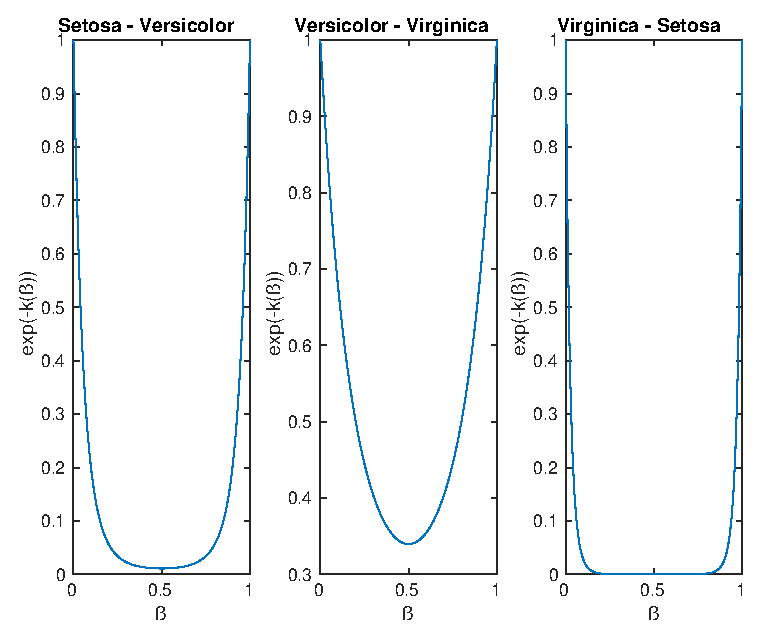
\includegraphics{errorCaseA}
 \caption{Case A - Error bound}
 \label{case a error}
\end{figure}

The experimental error was also examined for the data set.

\begin{table}[htb]
\begin{center}
\begin{tabular}{ll}
$P_{12}$ & 0.000\%\\
$P_{23}$ & 4.000\%\\
$P_{31}$ & 0.000\%
\end{tabular}
\end{center}
\caption{Case A - Experimental error}
\label{tab: case a experiment}
\end{table}


% errorExp =
%
%          0    0.0400         0

\newpage
\pagebreak

\subsection{Case B}

For this case, the Chernoff bounds were determined to be

\begin{table}[htb]
\begin{center}
\begin{tabular}{ll}
$P_{12}$ & 0.0049\%\\
$P_{23}$ & 6.3073\%\\
$P_{31}$ & 0.0000\%
\end{tabular}
\end{center}
\caption{Case B - Chernoff Bound}
\label{tab: case b chernoff}
\end{table}

Likewise the Bhattacharyya bounds were determined


\begin{table}[htb!]
\begin{center}
\begin{tabular}{ll}
$P_{12}$ & 0.0049\%\\
$P_{23}$ & 6.3073\%\\
$P_{31}$ & 0.0000
\end{tabular}
\end{center}
\caption{Case B - Bhattacharyya Bound}
\label{tab: case b bhatt}
\end{table}


\begin{figure}
 \centering
 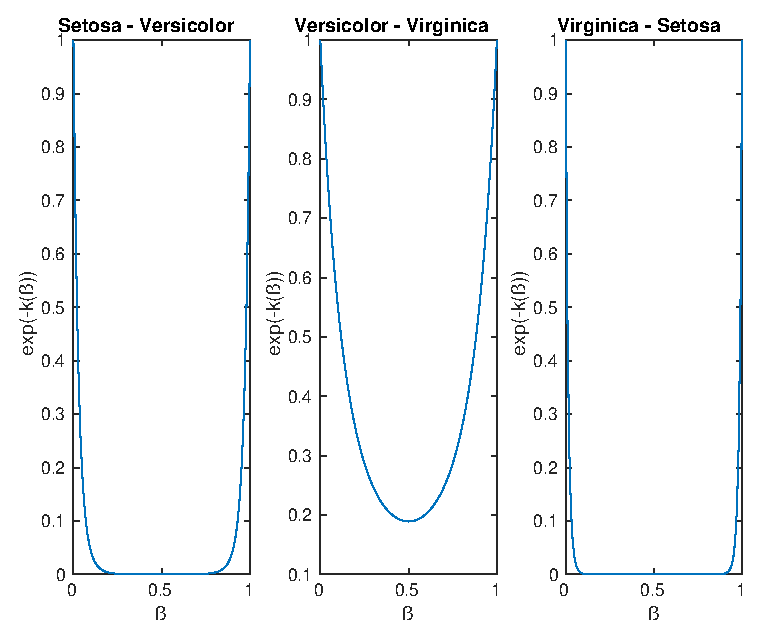
\includegraphics{errorCaseB}
 \caption{Case B - Error bound}
 \label{case b error}
\end{figure}


The experimental error was also examined for the data set.

\begin{table}[htb]
\begin{center}
\begin{tabular}{ll}
$P_{12}$ & 0.000\%\\
$P_{23}$ & 8.000\%\\
$P_{31}$ & 0.000\%
\end{tabular}
\end{center}
\caption{Case B - Experimental error}
\label{tab: case b experiment}
\end{table}

% errorExp =
%
%          0    0.0800         0

\newpage
\pagebreak

\subsection{Case C}

For this case, the Chernoff bounds were determined to be

\begin{table}[htb!]
\begin{center}
\begin{tabular}{ll}
$P_{12}$ & 0.0012\%\\
$P_{23}$ & 7.9909\%\\
$P_{31}$ & 0.0000\%
\end{tabular}
\end{center}
\caption{Case C - Chernoff Bound}
\label{tab: case c chernoff}
\end{table}

Likewise the Bhattacharyya bounds were determined


\begin{table}[htb!]
\begin{center}
\begin{tabular}{ll}
$P_{12}$ & 0.0074\%\\
$P_{23}$ & 8.0726\%\\
$P_{31}$ & 0.0000\%
\end{tabular}
\end{center}
\caption{Case C - Bhattacharyya Bound}
\label{tab: case c bhatt}
\end{table}

\begin{figure}
 \centering
 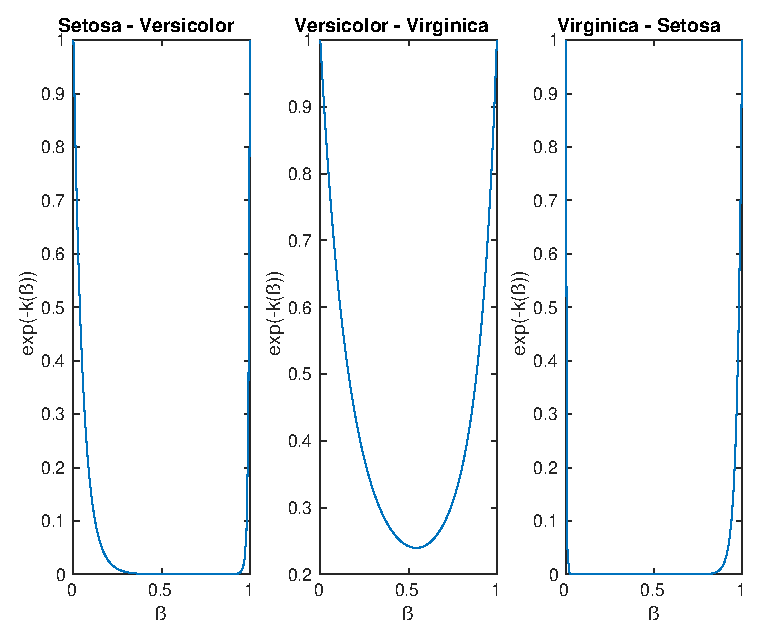
\includegraphics{errorCaseC}
 \caption{Case C - Error bound}
 \label{case c error}
\end{figure}

The experimental error was also examined for the data set.

\begin{table}[htb]
\begin{center}
\begin{tabular}{ll}
$P_{12}$ & 0.000\%\\
$P_{23}$ & 3.333\%\\
$P_{31}$ & 0.000\%
\end{tabular}
\end{center}
\caption{Case C - Experimental error}
\label{tab: case c experiment}
\end{table}


% errorExp =
%
%          0    0.0333         0
